\documentclass[12pt]{article}
%Gummi|065|=)

\usepackage{amsmath}
\usepackage{amsfonts} 
\usepackage{hyperref}
\usepackage{color}
\usepackage{graphicx}
\usepackage{float}
\usepackage{svg}
\usepackage{pagecolor}
\usepackage[most]{tcolorbox}

\textheight = 20 cm

\definecolor{blueColor}{HTML}{0069f5}



\begin{document}

\newpage

\pagecolor{blueColor}

\begin{titlepage}
    \centering

     
\includegraphics[width=0.88\textwidth, keepaspectratio]{arka-cover.png}
    
\end{titlepage}

\newpage

\pagecolor{white}




\renewenvironment{abstract}
 {\small
  \begin{center}
  \bfseries \abstractname\vspace{-.5em}\vspace{0pt}
  \end{center}
  \list{}{
    \setlength{\leftmargin}{.5cm}%
    \setlength{\rightmargin}{\leftmargin}%
  }%
  \item\relax}
 {\endlist}
 

\title{\textbf{Pairfy,\\A P2P ecommerce protocol based on trust rating and blind peers. }}
\author{Juan C. Rey\footnote{@pairfy  website: \url{www.pairfy.io} }\\}


\maketitle

\renewcommand*\abstractname{\textbf{}\hfill}
\abstract{
\textbf{Abstract.} Pairfy is an electronic commerce protocol that uses smart contracts to decentralize functional requirements necessary for the processes of selling and buying a physical product.
Any member of the community can post a product for sale and any member of the community can express an intention to purchase that product.
If the stock of a product is 15, only the 15 fastest people who express their intention to buy will be able to occupy a slot and secure a negotiation session.
The slot of a product is a concept that represents the availability to open a negotiation session similar to a sell order on a DEX. A slot can be released if the buyer or seller cancels the session.
A negotiation session is defined as the process of trading a product for a limited time. The buyer and seller generate the negotiation context by engaging in bilateral communication.
}


\section{Introduction}

Pairfy is an electronic commerce protocol that uses smart contracts to decentralize functional requirements necessary for the processes of selling and buying a physical product.
Any member of the community can post a product for sale and any member of the community can express an intention to purchase that product.
If the stock of a product is 15, only the 15 fastest people who express their intention to buy will be able to occupy a slot and secure a negotiation session.
The slot of a product is a concept that represents the availability to open a negotiation session similar to a sell order on a DEX. A slot can be released if the buyer or seller cancels the session.
A negotiation session is defined as the process of trading a product for a limited time. The buyer and seller generate the negotiation context by engaging in bilateral communication.



\section{ Requirements }

The functional requirements for the operation of the protocol are: Negotiation session, State machine, Blind peers.

\subsection { Negotiation session }

The negotiation session is a 4-stage synchronous process \emph{Waiting}, \emph{Locking}, \emph{Delivery}, \emph{Finish}. A stage cannot start if the previous stage has not finished, the transitions are sequential not parallel.

\subsubsection { Waiting }

\begin{figure}[ht]
  \centering
  \includesvg[width=0.86\textwidth]{waiting.svg}
  \caption{Script deployment}
  \label{fig:mi_imagen}
\end{figure}


When a seller offers a product to the public by activating a slot (sale order) a small plutus script with state machine logic is activated in the blockchain.
The seller must lock an amount greater than 0 ADA as collateral. 
If the seller acts in bad faith during the negotiation session the seller will lose the collateral.
If the seller is a good agent during the negotiation session the collateral will return to him.
Collateral guarantees that the seller behaves honestly.
This mechanism of coercion allows to generate trust in potential buyers. 
It also allows the seller to increase their trust rating. Example. Alice publishes a book with 20 units of stock.
She activates only 10 slots (sale orders) each with a collateral of 20 ADA.
In the first few hours 7 books were sold and now there are only 3 slots left.
Alice decides to activate the 10 remaining slots due to demand.
Bob sells the same product with the same stock but offers collateral of 5 ADA. The community prefers to buy the books from Alice since she is more committed to fulfilling her obligation by offering 20 ADA collateral.
Other factors increase the seller's trust rating such as the total number of successful sales, seniority, or profile information.
In the background for each activated slot individual scripts are deployed on the blockchain waiting to be occupied by buyers.

\subsubsection { Locking }

\begin{figure}[ht]
  \centering
  \includesvg[width=0.86\textwidth]{locking.svg}
  \caption{Session locked}
  \label{fig:locking}
\end{figure}


In Figure 2 you can see the collateral of 50 ADA given by the seller and the price of the product 100 ADA given by the buyer.
When the buyer presses the buy button a slot is occupied and the state of the script transitions from \emph{Waiting} to \emph{Locking}.
Blocking funds allows participants to advance their obligations.
The seller's obligation is to deliver the correct product with the correct specifications. The buyer's obligation is to receive the product and pay the price.
It is important to clarify that the buyer's obligation to pay the price is guaranteed when he occupies a slot since the amount in ADA of the product price is a necessary condition to occupy a slot.

From this point the seller can start with questions such as: What is the delivery point? Description of delivery point? Any questions necessary to guarantee the effective delivery of the product.

All information provided by both actors in the user interface is contained within a websocket instance and can only be observed by the blind peers in case of a dispute.
The websocket server does not store any type of information about the negotiation session once legal security is declared about the business between the parties.
Legal security is declared by the blind peers and refers to the absence of reasonable doubt in the fulfillment of the obligations corresponding to the buyer and the seller.


\subsubsection { Delivery }


\begin{figure}[ht]
  \centering
  \includesvg[width=0.86\textwidth]{delivery.svg}
  \caption{Delivery confirmed by seller}  
  \label{fig:delivered}
\end{figure}



When the shipping company confirms the effective delivery of the product the seller can invoke the @delivered endpoint.
The script transitions from \emph{Locking} to the \emph{Delivery} state which indicates that the seller has fulfilled its delivery obligation.
Finally, the buyer confirms whether he received the product by invoking the @received endpoint. By doing so, the script transitions to the last state \emph{Finish} which releases the funds to the seller's wallet.
\subsubsection { Finish }

\begin{figure}[ht]
  \centering
  \includesvg[width=0.86\textwidth]{finish.svg}
  \caption{Delivery confirmed by buyer}
  \label{fig:delivered}
\end{figure}




\subsection { State machine }

A state machine also known as a finite state machine (FSM), is a mathematical model used to describe the behavior of a system or process that can exist in a limited number of distinct states. The system transitions from one state to another in response to specific events or input conditions, and these transitions are defined by a set of rules or conditions known as transitions.

A deterministic finite state machine (DFSM) is a specific type of state machine that exhibits deterministic behavior, meaning that for any given state and input, there is a unique and unambiguous next state. In a deterministic state machine, the transition from one state to another is uniquely determined by the current state and the input with no ambiguity or randomness involved.

\begin{figure}[ht]
  \centering
  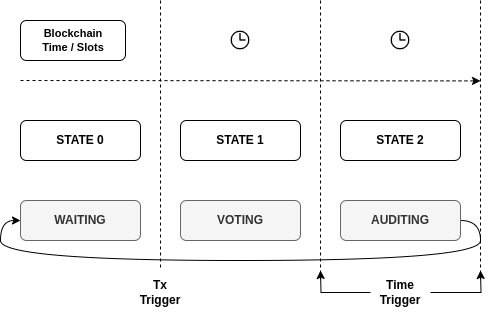
\includegraphics[width=0.95\textwidth]{machine.png}
  \caption{Session states}
  \label{fig:States}
\end{figure}

Figure 5 shows the deterministic state machine concepts applied to the steps of a negotiation session. Contracts in Cardano's EUTXO model need at least one initial transaction to trigger their design logic and configure its initial state. When the seller activates a slot his wallet deploys a plutus script that receives the collateral in ADA and necessary parameters for the session. 
\\

\begin{tabular}{lr}
\textbf{sessionState} \emph{:: SessionState}\\
\textbf{sessionState}  = SessionState  \textbraceleft{}
\\ \hspace{55mm}cState = 0
\\ \hspace{55mm}sLabel = ``waiting"
\\ \hspace{55mm}tDuration = 100
\\ \hspace{55mm}cSlot = False
\\ \hspace{55mm}pDelivered = False
\\ \hspace{55mm}pReceived = False
\\\hspace{51mm}\textbraceright{} 
\end{tabular}
\\

 The data type \emph{sessionState} represents the initial state of the plutus script once deployed by the seller. These variables will remain in the default state indefinitely until the buyer's wallet interacts with the script taking the slot.
\\

\begin{tabular}{lr}
\textbf{sessionState} \emph{:: SessionState}\\
\textbf{sessionState}  = SessionState  \textbraceleft{}
\\ \hspace{55mm}cState = 1
\\ \hspace{55mm}sLabel = ``locking"
\\ \hspace{55mm}tDuration = 100
\\ \hspace{55mm}cSlot = True
\\ \hspace{55mm}pDelivered = False
\\ \hspace{55mm}pReceived = False
\\\hspace{51mm}\textbraceright{} 
\end{tabular}
\\

 \emph{cSlot} represents the variable that indicates whether the script has been occupied by a buyer. The boolean value True means that the slot has been occupied by a buyer which makes the script transition from \emph{Waiting} to \emph{Locking}.
\\

\begin{tabular}{lr}
\textbf{sessionState} \emph{:: SessionState}\\
\textbf{sessionState}  = SessionState  \textbraceleft{}
\\ \hspace{55mm}cState = 2
\\ \hspace{55mm}sLabel = ``delivery"
\\ \hspace{55mm}tDuration = 100
\\ \hspace{55mm}cSlot = True
\\ \hspace{55mm}pDelivered = True
\\ \hspace{55mm}pReceived = False
\\\hspace{51mm}\textbraceright{} 
\end{tabular}
\\

\emph{pDelivered} is a variable of type boolean that represents the delivery of the product or not. 
At this point the seller has invoked the @delivered endpoint stating that he has fulfilled his obligation to deliver the product. This action makes the script transition from \emph{Locking} to \emph{Delivery}
\\

\begin{tabular}{lr}
\textbf{sessionState} \emph{:: SessionState}\\
\textbf{sessionState}  = SessionState  \textbraceleft{}
\\ \hspace{55mm}cState = 3
\\ \hspace{55mm}sLabel = ``finish"
\\ \hspace{55mm}tDuration = 100
\\ \hspace{55mm}cSlot = True
\\ \hspace{55mm}pDelivered = True
\\ \hspace{55mm}pReceived = True
\\\hspace{51mm}\textbraceright{} 
\end{tabular}
\\

\emph{pReceived} is a boolean variable that represents whether the buyer confirms receipt of the product or not. This variable is modified only by the buyer using the @received endpoint.
By doing this, the script transitions to its final state \emph{Finish} which releases the funds to the seller.
 
 
\subsection { Blind peers }  

Connecting the blockchain to the real world is an expensive challenge at least for physical commodity trading.
Shipping companies would have to connect their vehicles to supervised oracles.
The products must have an infallible tracker to check if the product was delivered.
A lot of infrastructure deployed around the world is necessary to achieve a fully decentralized ecommerce protocol. This represents a very difficult challenge to achieve, another option is to use the human brain as a source of truth.
With the right conditions the human brain can make logical reasoning about facts or propositions to declare a truth.
For example, the peer review system in the academic world allows a research paper to be reviewed by other experts randomly. A blind reviewer does not know who is the author of the paper he is reviewing. The author also does not know who the reviewers are.
The system maintains confidentiality to prevent biases, ensuring a rigorous and impartial assessment. Serving as a crucial quality control mechanism, it identifies errors, provides constructive feedback to authors, and contributes to the overall accuracy and reliability of published work. 
A system of blind peers trained in conflict resolution can decide on a dispute in a negotiation session in the event that the buyer or seller fails to comply with their obligations or another problem arises that does not allow the natural conclusion of the session.
A blind peer system can decide on a disputed trading session.

\subsubsection { Appeal } 

\emph{Peer-to-Peer} cryptocurrency exchange services such as localbitcoins or binance P2P have proven to be systems that work for secure exchanges. These systems are based on trust ratings and involve real-world action on the part of the buyer such as making a transaction to the bank account provided by the seller.

In Binance's P2P disputes between buyers and sellers can be addressed through an appeal process. Common reasons for initiating an appeal involves problems with payment confirmation, disagreements over payment quality, or disputes regarding trade terms. To protect the cryptocurrency involved in the trade an escrow system locks the funds.

Both the buyer and seller are afforded the opportunity to present evidence or explanations supporting their case during the appeal. A mediation team at Binance reviews the appeal, carefully considering the evidence and arguments put forth by both parties. Subsequently, Binance reaches a decision which may involve upholding the original trade agreement, releasing funds from escrow to the appropriate party, or taking other actions based on the specific circumstances of the dispute.






















In the blockchain industry new projects are created daily and the auditable list of projects will inevitably grow over time. It is possible for the community to add 1000 or 10000 projects if they wish. The consequence of this is the large number of indexes in the database. Managing such a number of indexes in a smart contract can be challenging because the limit of Kb per Tx is limited and it is not scalable. However, we can simplify the notion of long-length indices such as those used in databases by using consecutive natural numbers.

A 32-bit unsigned integer can be represented as 0 to 2147483647. A positive integer can be assigned as a unique index to each project added by the community in ARKA. In this way a smart contract could reference a large number of projects using only 32 Bits. For example, an user wants to vote for the project called Minswap which has the index 742 assigned, no other project has this index. The user connects their wallet containing the ARKA utility token to the UI and performs the vote. The request goes to the backend and contract integration calling the endpoint \emph{createVote} that receives a 32-bit positive integer as a parameter. The contract verifies if the parameter is valid and if the UTxO associated with that wallet address contains the ARKA token. The contract finally checks if the index given as a parameter is less than or equal to \emph{tProjects} variable of the contract which refer to the total number of projects in the auditable list. If these conditions are correct the contract validates the Tx and adds a small mark in the metadata.


Once the \emph{Voting} stage is finished a snapshot is taken at the exact moment or Slot in which the stage ends. By making a query to the blockchain API it is possible to get the transactions associated with the address of the contract to validate the status of the transactions, verify if the transactions have been validated by the contract and verify the metadata of the transaction that provides the context resulting from the interaction with the contract. The metadata can help in identifying the purpose and status of the transaction. The information about the snapshot and governance stage is displayed in the platform UI for all users.

This configuration for the voting system guarantees speed, minimum computing time and the ability to validate millions of indexes using a simple condition:

$\emph{indexParam} \leq \emph{tProjects}$  $\Rightarrow$ \text{True}. Where \emph{indexParam} is the parameter sent by the user and \emph{tProjects} is the total number of projects on the auditable list.

\begin{figure}[ht]
  \centering
  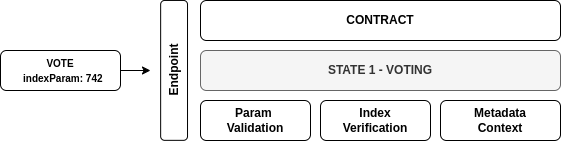
\includegraphics[width=0.85\textwidth]{vote.png}
  \caption{Voting
  }
  \label{fig:mi_imagen}
\end{figure}

The parameter \emph{tProjects} can be added by the operational wallet when calling the \emph{startRound} endpoint. This parameter within the smart contract corresponds to a positive integer number. For example, in case there are 1032 projects listed by the community \emph{tProjects} will be 1032. In the initial state of the contract this variable value is 0. At the end of the governance stage this variable will also be 0.

In the hypothetical case that the contract itself was designed to store the project indices in the form of assets or NFTs to later be consulted in the governance stage, this would add more logic to the contract and therefore computation time. For this reason it is a disadvantage to use the contract as a form of storage.

However, it is possible to assign a simple time-locked plutus script that allows to store the indices with project names in the form of small metadata using assets (1 asset per project) or simply stamping valid transactions without using assets. The operational wallet is the only one that will be able to interact with this plutus script. The address of the script on the blockchain will need to be included in the metadata when deploying the ARKA contract for the first time for auditability. This solution is scalable since multiple scripts can be used for this purpose. In this way there is complete audability with respect to the indices. Another form of index auditability is public code repositories like Github or distributed storage systems like IPFS. In future iterations of the V1 contract it is possible to add a new stage where the community can add projects to the auditable list using voting.

\subsection { Random assignment }
   
Assigning auditors to auditable projects can be a point of low auditability if it is done centrally on private servers. For that reason the best option is a decentralized assignment algorithm. There is not much complexity in the logic required for an equal assignment for all auditors. The main requirements are randomness and uniform distribution of the probability of being chosen as an auditor of a project. The fisher-yates algorithm is a great candidate because it ensures that each element has an equal probability of being placed in any position of the resulting permutation. This is useful since it can shuffle a finite list of indices. For example, \emph {A = [0...50]} where \emph {A} is the list of indices from auditor 0 to auditor 50. Each index represent a specific auditor and they are ordered consecutively [0,1,2,3,4...50]. When the algorithm is applied to the list the positions of the indices will change randomly. If ARKA needs 12 auditors for an audit round the first 12 indices from the shuffled list will be selected.\\

1. \emph {auditorPool } = [0,1,2,3,4...50] \\
2. \emph {auditorPoolShuffled } = [30, 13, 10, 19, 21, 45, 23, 47, 31, 50,  4, 28, ... 34]\\
3. \emph {selectedAuditors} = [30, 13, 10, 19, 21, 45, 23, 47, 31, 50,  4, 28]\\
4. \emph {auditorGroups } = [ [30, 13], [10, 19], [21, 45], [23, 47], [31, 50],  [4, 28] ]\\

The auditors are randomly selected using the Fisher-Yates algorithm and finally grouped. ARKA requires 2 auditors per project so in this example there are 6 groups for the first 6 projects chosen by the community through voting. The permutations occur on all indexes so there is no need to perform new permutations for role assignment or grouping.


\begin{figure}[ht]
  \centering
  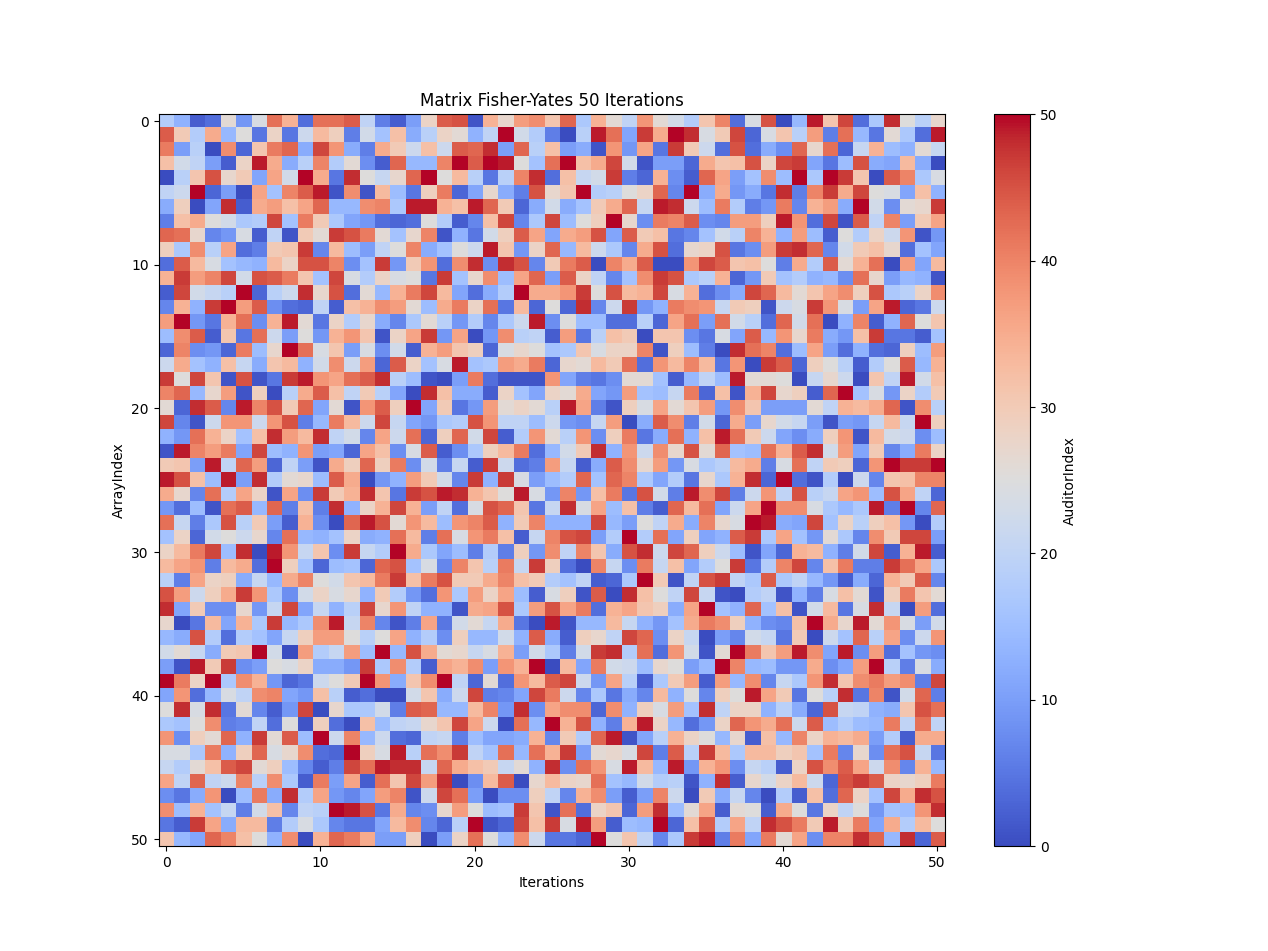
\includegraphics[width=1\textwidth]{haskell-matrix.png}
  \caption{Haskell
  }
  \label{fig:haskell-matrix}
\end{figure}


\begin{tcolorbox}[title=Haskell Code]
\begin{verbatim}

{-# LANGUAGE OverloadedStrings #-}
import System.Random (randomRIO)


shuffle :: [Int] -> IO [Int]
shuffle [] = return []
shuffle xs = do
  let m = length xs - 1
  random <- randomRIO (0, m)
  let (left, (chosen:right)) = splitAt random xs
  shuffledRight <- shuffle (left ++ right)
  return (chosen : shuffledRight)


\end{verbatim}
\end{tcolorbox}


This Fisher-Yates haskell version can be used as a reference to create a plutus implementation. The code inside a plutus contract is deterministic it is necessary to use an oracle that generates a random number for the \emph {random} variable or use a pseudo random number generator (PRNG) that takes the hash of the last block generated by the blockchain as a seed of entropy.

\subsection { Report Minting }

The auditor report and its respective review are two different but necessarily related resources they make up a complete audit report. To ensure the immutability of its content it is necessary mint them as non-fungible assets. This can be done automatically from the backend integration at the end of the \emph{Auditing} stage. 
The latest version of the .json documents sent by the auditor and the reviewer will be hashed to subsequently mint 3 copies. 1 NFT will be sent to the wallet provided by the auditor. Another will be sent to the reviewer's wallet and another will be stored in a wallet of the DAO. They will be stored in IFPS and Github.

This mechanism can be implemented in the smart contract for its operation during the \emph{Auditing} stage. For example, supplying the contract with the list of wallets that have authorization to mint and some status variables to indicate if they have already minted their report or not. Or use identity tokens as a form of authorization to mint. However this will be the subject of investigation for future versions of the smart contract.


\section{ Levels of certification }


\subsection { Fundamental }


\subsection { Tested }


\subsection { Formal verification }


\section{ Auditors }

The auditors are in charge of creating and reviewing the reports in the \emph{Auditing} stage. They are elected by the community using governance. They have the ability and experience to generate high-quality reports.

\subsection { Sandbox }

It is a practice environment for potential auditors and amateur researchers. It is a 1:1 workspace used by auditors in audit rounds. Users can conduct research according to the question scheme and generate high-quality reports with the tools provided by LaTeX. The purpose of the sandbox is multiple, train future auditors and provide reports to the community. Anyone can use this environment.


\subsection { Designation }

The community is in charge of choosing the auditors using the \emph{ARKA} governance token. Anyone can apply if they have previously made 3 reports in the sandbox. The election is completely decentralized.
 

\subsection { Pool }

The auditor pool is a unique list of official \emph{ARKA} auditors. An auditor has 2 states, available and not available. Available auditors are those who have expressed interest in participating in the current audit round. Only auditors that have been declared as available can be assigned to auditable projects depending on the random assignment algorithm of the smart contract. A function of the algorithm randomly selects the available auditors and creates groups. \emph{Group = [ auditor, reviewer ]}. The groups are assigned to the projects previously voted on in \emph{Voting} stage. After this process, everything is ready for the \emph{Auditing} stage to start. 


\section { Tokenomics }











\end{document}
